\lab{Multi-Armed Bandit Problems}{Multi-Armed Bandit Problems}
\objective{This lesson explains Markov decision processes --
specifically multi-armed bandit problems -- and how to solve them by
Thompson Sampling. An application to web page experiments is addressed.}

\section*{Markov Decision Processes}
Previously we considered dynamic programming problems.
These problems involve making sequential decisions in some optimal way,
while dealing with possible uncertainties.  Dynamic programming problems are closely
related to a class of problems called Markov Decision Processes.

A Markov Decision Process (MDP) involves the following elements:

\begin{itemize}
\item   A set of decision times,
\item   A set of states,
\item   A set of actions,
\item   A set of rewards dependent on the state and action, and
\item   Transition probabilities dependent on states and actions.
\end{itemize}
In this lab we will consider discrete time problems, so that our
set of decision times is $t = 1,2,3,\ldots$.
\begin{comment}
In the dynamic programming problems considered in the previous labs,
the set of states was the set of all possible levels of wealth and
the actions were how much wealth to save for the next period.
The rewards were given by the utility function $u(\cdot)$,
and we considered both deterministic and stochastic transitions.
\end{comment}
\section*{Bandit Problems}
In particular, we will consider what is called the multi-armed bandit
problem.  The name comes from the following example.
Suppose there is a row of $N$ slot machines (``one-armed bandits")
where probability of winning is $p_i$, $i= 1,2,\ldots,N$,
and these probabilities are unknown to the gambler.
The gambler seeks to determine the sequence of levers to pull in
order to maximize her winnings.

Bandit problems have a wide range of applications.
One can consider the ``arms" to be the different treatments in a
clinical trial, the different forms of advertising a product,
or the different research projects a company might invest in.

We now formulate the multi-armed bandit problem precisely.
For simplicity, suppose there are $2$ arms, although the
discussion can easily be extended to $N$ arms.
Any one arm can be pulled in each time period $t= 1,2,\ldots$.
With unknown probability $p_i$, the $i$-th arm gives
reward $1$ and with probability $1-p_i$ it gives reward $0$.
Note we have now defined a set of decision times, actions, and rewards.
We define the state to be a 4-tuple giving the number of successful and unsuccessful
pulls on each arm up to that point, written as
\begin{equation}\label{state}
(a_1,b_1,a_2,b_2),
\end{equation}
where $a_i$ is the number of successful pulls on arm $i$ and $b_i$
is the number of unsuccessful pulls on arm $i$.
As we pull the arms, we must balance between pulling the arm that has
the highest expected payoff and pulling all arms in order to gain
information about the probabilities $p_i$.
This trade-off is often referred to as exploring versus exploiting.
In essence, while gaining rewards, we will also come up with
better estimates for the real values of each $p_i$, which will improve our decision making.
We will do so by Bayesian updating.

\section*{Bayesian Updating}
While a full exposition of Bayesian inference is well beyond the
scope of this lab, the essential concepts are fairly straightforward.
We recognize that we do not know the values of the $p_i$,
but given our past history of successful and unsuccessful
pulls, we can say something about what range we think they might be in.
This is different than guessing a specific value for the $p_i$.
Instead of specifying what we think is the most likely value of $p_i$,
we can encode our knowledge of and uncertainty about $p_i$ in a
probability distribution,
like those seen in Figure \ref{fig:priors}.
\begin{figure}

\centering
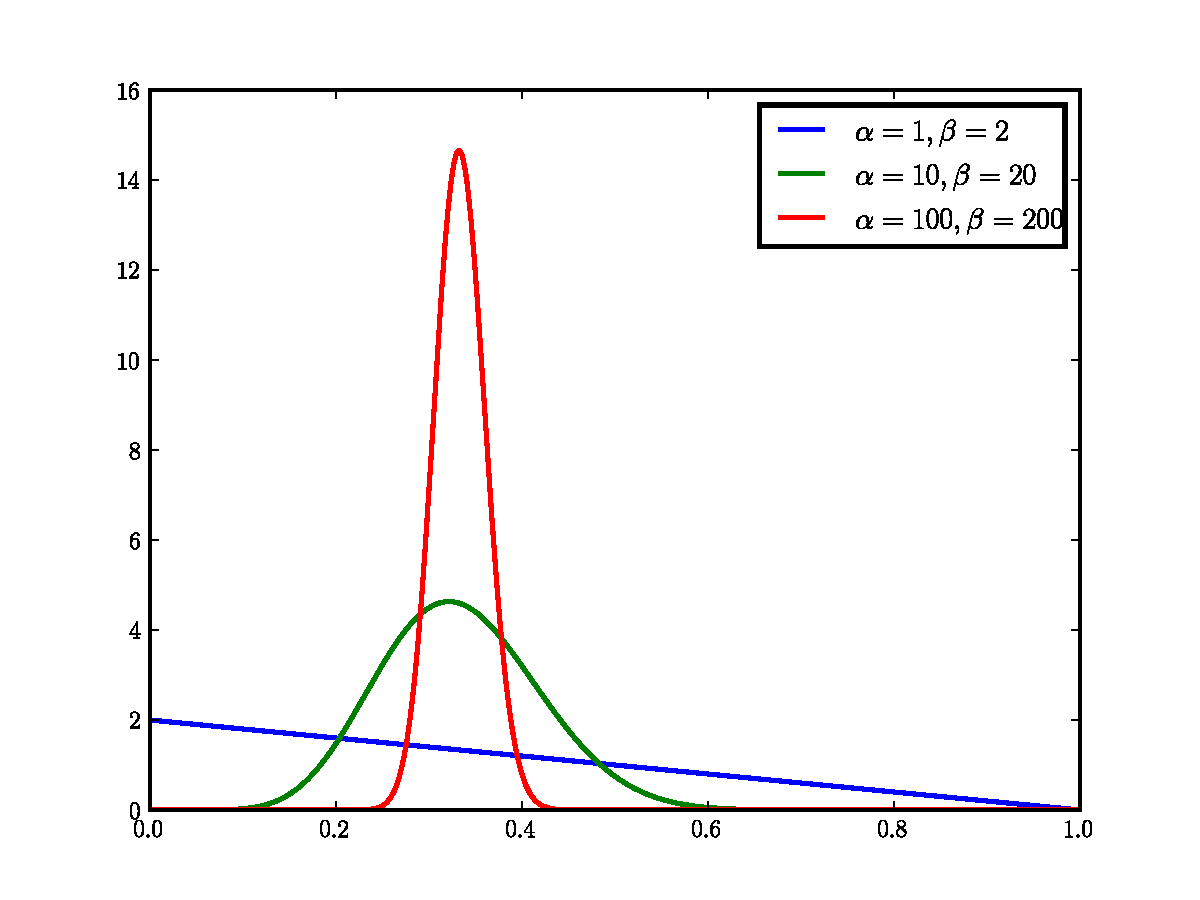
\includegraphics[width=\textwidth]{priors.pdf}
\caption{Bayesian priors}
\label{fig:priors}
\end{figure}

If you have had $1$ success and $2$ failures, you might
think that the success probability
$p_i$ is around $\frac{1}{3}$.
However, you have very little information at this point,
so rather than assuming the exact value for $p_i$,
you might represent your belief about $p_i$
by the blue probability distribution in Figure \ref{fig:priors}.
We call the distribution that describes our belief about $p_i$
the \emph{prior distribution} of $p_i$.  If we incorporate new information,
we get a new distribution, called the \emph{posterior distribution}.
As we collect even more information, the posterior distribution becomes
the new prior distribution. This framework allows us to fluidly incorporate
new information as we seek to determine the value of $p_i$.

As we get more information, the probability curve gets narrower.
In the figure, we see that the distributions have expected
value of $1/3$ and become tighter around that value.
This is fitting since the parameter values are successful one third (computed by $\alpha/(\alpha+\beta)$)
of the time, and the tighter distributions correspond to having
more prior information.  If we need an estimate for $p_i$, we can use
the expected value of our distribution corresponding to $p_i$.
We will denote this estimate by $\overline{p_i}$.

We will use this Bayesian framework in our approach to the multi-armed bandit problem.
We do not know the $p_i$, but each time we pull an arm, we update our distribution of
where we think it might be.
In particular, we use a beta distribution for each $p_i$.
A beta distribution is a continuous probability distribution on the interval $[0,1]$,
which corresponds nicely to the possible values of the $p_i$.  Beta distributions have
two parameters (given by $\alpha$ and $\beta$ in the figure).

In our problem, the state (given by \eqref{state}) can be thought of as representing two
beta distributions -- one for each $p_i$ with parameters $a_i$ and $b_i$.
The details of the updating process are unimportant for now, except
for this important property: the two parameters for the beta distribution
correspond exactly with successes and failures.
So if we start with a prior distribution Beta$(a,b)$ and the next pull is success,
our posterior distribution is Beta$(a+1,b)$. If the next pull is a failure, however, then
the posterior distribution is Beta$(a,b+1)$.
Observe how this corresponds with the way our state evolves.

\section*{Simulation and Sampling in a Bayesian Framework}
Along with the estimate $\overline{p_i}$, we can also compute many other useful
quantities in our Bayesian problem via random sampling.  Essentially, we can take
random draws from our distribution and estimate the mean, median, or other
quantities based on the value of those quantities in the random sample.
This is a very powerful concept that will be explored in more detail in future labs.

\begin{problem}
Write a function \li{sim\_data} that accepts an $n\times 2$ array, where each
row represents the parameters of a beta distribution, respectively, and a positive integer $k$
that represents the number of random draws to return.
The function should return a $k\times n$ matrix where each row has a random sample
from each of the $n$ arms.  This can be accomplished with ease using the NumPy function
\li{numpy.random.beta}.
\label{prob:simdata}
\end{problem}

\begin{comment}
\begin{problem}
Suppose one of the arms in a bandit problem has the state (or prior distribution of $p_i$)
Beta$(100,200)$ corresponding to $100$ successes and $200$ failures.
Simulate 10,000 data points for the distribution Beta$(100,200)$.
Compute $\overline{p_i}$ by finding the mean of the simulated points.
Compute the median.  Also compute the $95$th percentile using the command
\li{scipy.stats.mstats.mquantiles(data, .95)} where \li{data} is the array
containing the 10,000 simulated data points.
\end{problem}
\end{comment}
\section*{Direct Dynamic Programming Solution}
This framework lends itself well to a dynamic programming type solution.
We introduce the value function $R$ that depends on the state, and gives
the optimal expected value that can be achieved
starting from the state.  Then we have
\begin{equation}
\label{recurs}
\begin{aligned}
R(a_1,b_1,&a_2,b_2) =\\
 \max&\left\{\overline{p}_1\cdot[1 + \beta R(a_1+1,b_1,a_2,b_2)] +
 (1-\overline{p}_1)\beta R(a_1,b_1+1,a_2,b_2)\right. ,\\
&  \left.\overline{p}_2\cdot[1 + \beta R(a_1,b_1,a_2+1,b_2)] +
(1-\overline{p}_2)\beta R(a_1,b_1,a_2,b_2+1)\right\}
\end{aligned}
\end{equation}
The two terms in the maximization represent the expected value of pulling lever
one or lever two respectively.  For example, by pulling lever one, we expect
to get a reward of 1 with probability $\overline{p_1}$.
We must also account for the expected value of future rewards
(discounted by $\beta$) moving to a state with one more success on arm 1.
Note that this $\beta$ is not the same as that in our distribution, but is the discount
factor, as it was in the Value Function and Policy Function Iteration labs.
With probability $1-\overline{p_1}$, lever one does not give a reward and so
rewards are simply the discounted expected reward starting in the next state.

Notice that the expressions inside of $R(\cdot)$ on the right side have parameter
values that add to one greater than the $R(\cdot)$ on the left side.
So if we want to compute $R(1,1,1,1)$ we need to know
$R(2,1,1,1)$, $R(1,2,1,1)$, $R(1,1,2,1)$ and $R(1,1,1,2)$
(all possible combinations of parameters that add up to 5, 
which differ from the left hand side by a total value of one in exactly one position).
To compute these, we need to know the reward corresponding to all possible
combinations of parameters that add up to 6, and so on.  Consequently, we could
make a guess for all $R$ for all parameter combinations that add up to some large $N$,
then work backward until we get to $R(1,1,1,1)$.  This is backward induction,
just as we saw in dynamic programming.  However, the number of computations in this
problem grow much too quickly because of the branching nature of having multiple arms.
In fact, if there are more than two arms this method of computation is infeasible!


\begin{comment}
\section*{Gittins Index Solution}
One way we might hope to solve a bandit problem is by computing some sort of ``index''
for each arm.  That is, we want a number associated with each arm that in some sense
captures the value of pulling that arm.   Ideally such an index would depend only on that arm,
and not on the others.  We could then compare the indices for all of the arms
and pull the arm with highest index.  It turns out that bandit problems can be
solved optimally by such methods and are computationally more feasible than the
dynamic programming approach we saw above.

To compute an index for this problem, we consider comparing an arm with unknown
payoff probability $p_i$ to an arm with known payoff probability $p$.  Then equation \eqref{recurs}
becomes
\begin{equation}\label{index}
\begin{aligned}
R(p,a_i,b_i) = \max&\left\{\frac{p}{1-\beta} \right. ,\\
&  \left.\hat{p}_i\cdot[1 + \beta R(p,a_i+1,b_i)] + (1-\hat{p}_i)\beta R(p, a_i,b_i+1)\right\}.\\
\end{aligned}
\end{equation}

We determine the expected value of pulling the first arm to be $\frac{p}{1-\beta}$
noting that if we pull the deterministic arm once, we will continue pulling it
forever as we gain no new information.  In this case the expected reward from pulling
the known arm is $p + \beta p + \beta^2 p + \cdots = \frac{p}{1-\beta}$.


If we can find the $p$ such that we are indifferent between the deterministic
arm and the unknown arm, this will give us an index that quantifies the value of arm $p_i$
(this can be proved).

Putting all of this together, our algorithm for solving the multi-armed bandit
problem with two arms is as follows.  For each arm $i$, compute \eqref{recurs}
over a range of $p$ values to find the $p$ such that you would be indifferent
between the arm with probability $p$ and arm $i$. Store this as the index $\lambda_i$.
Compare the $\lambda_i$ and pull the arm with largest index.

In order to compute \eqref{index} we use dynamic programming, starting with a guess
for $R$ for parameters that add up to some large $N$ and use backward induction.
In the process, we find $R$ and $\lambda_i$ for each combination of parameters
that adds up to any $n\leq N$. Thus we do not have to compute new $\lambda_i$ after
each pull, we can just look them up.

\section*{Algorithm Outline}
This section will guide you through creating a function that will compute the indices
for a given arm.  It will involve writing a number of functions that you can save in the same
.py file.

First, we need a function that will compute all the pairs of $a,b$ that add up
to some $N$.  We also want the user to be able to input the minimum values of
$a$ and $b$ of interest to avoid unnecessary computation.  For example if in practice
all of the arms have $a_i \geq 5$ and $b_i \geq 10$, then we are uninterested in smaller $a$, $b$.
The following code accepts the value of $N$ and a minimum value of a and b and
returns an $N$ by 2 array with the $a$'s and $b$'s such that $a + b = N$.
\begin{lstlisting}
# computes pairs of numbers starting with mina and minb that
# add up to N

def compute_indices(N,mina,minb):
    import scipy as sp
    avec = sp.arange(mina,N-minb+1)
    avec = sp.reshape(avec,(avec.shape[0],1))
    bvec  = sp.arange(N-mina, minb-1,-1)
    bvec = sp.reshape(bvec,(bvec.shape[0],1))
    values = sp.hstack((avec,bvec))

    return values
\end{lstlisting}

In order to perform the backward induction, we need to be able to estimate the value
$R(p,a,b)$ for $a+b = N$.  To do so we have to estimate the second quantity in \eqref{index}.
We will estimate it as $(\frac{a}{a+b})/(1-\beta)$.  This is the value one would get by
pulling an arm with $p_i$ equal to the expected value of $Beta(a,b)$ forever.
\begin{problem}
Write a function ``end\_reward" that accepts $p,a,b,$ and $\beta$ and returns the
estimated value of $R(p,a,b)$ for $a,b$ such that $a+b=N$.
\end{problem}

For convenience it will be nice to have a function that will compute $R(p,a,b)$
given values of $p,\overline{p},a,b,\beta,N$ as well as values of $R(p,a+1,b)$ and $R(p,a,b+1)$.
This should follow directly from \eqref{index}.
\end{comment}

\section*{Thompson Sampling}
\begin{comment}
There is a method for computing the optimal solution to the multi-armed bandit problem
based on what is commonly known as the Gittins Index Theorem.
Computationally it is similar to the dynamic programming approach, but it is significantly less
costly.
Unfortunately, for large scale problems, it can still be too costly.
\end{comment}
There are, however, many heuristic methods of solving the multi-armed bandit problem.
In particular we will use a method known as Thompson Sampling, or Randomized Probability Matching.
The idea is that we should choose arm $i$ with probability equal to the probability
that arm $i$ is the best arm.  So if we believe there is an $80\%$ probability that
arm 2 is the best arm, we will pull it $80\%$ of the time.  The other $20\%$ of the
time we would pull arm one, which will help give more information about the true value of $p_1$.
In this way, we will pull most often the arms from which we expect the most rewards;
however, we will also pull other arms with some probability so that we accomplish some
exploration and gain information on all arms, until we are confident we have found the best arm.

\begin{problem}
Write a function \li{arm_probs} that accepts a $k \times n$ array of data computed by the
function from Problem \ref{prob:simdata}.

This function should return a vector of the probabilities that each of the $n$ arms is optimal.
This can be computed for each arm by determining how many of the total $k$ simulations
that arm had the highest value.  This value, the number divided by $k$, will give the proportion
of the simulations for which this arm had the greatest probability of success.
This proportion is interpreted as the probability that the arm is the optimal arm.
\end{problem}

In some applications, we might want to run computations once, then pull many arms instead
of computing before each pull.  In these cases, rather than computing these probabilities,
choosing an arm, then recomputing, it can be more convenient to view the probabilities as weights.
For example, we can view the probabilities as the weights of how to distribute the next 100 pulls.
Suppose the probabilities resulting from the previous function (with two arms) are $0.4$ and $0.6$.
Then we would allot 40 of the next 100 pulls to arm 1 and 60 of the next 100 pulls to arm 2.
Then we could compute new weights for the next 100 pulls.

\begin{problem}
Using the results from the previous problems, write a function \li{get_pulls} that determines how many
times each arm should be pulled in the next $M$ pulls, where $M$ is an input to the function.
The function should accept a vector of probabilities of the form returned by the
function in the previous problem, and a number of pulls $M$.
Note that you will have to round since the number of pulls for each arm must be in integer.
Return a vector of length $n$ (where $n$ is the number of arms) that gives the number of
pulls out of the next $M$ for each arm.  Make sure the entries sum to $M$.
\end{problem}

You now have code that solves the version of the multi-armed bandit problem described here.
We first start all arms with the state (or prior) Beta$(1,1)$,
which is the uniform distribution, meaning we have no information on the values for each $p_i$.
Then we compute the weights for the next $M$ pulls.
After those $M$ pulls, we compute new weights and continue on in this pattern.
In some applications we may not continue this forever, but might instead have some stopping
criterion for when we think we have identified the best arm.
A common stopping criterion is to stop when one of the arms has a $95\%$ probability
(or some other specified probability) of being the optimal arm.
In the framework we have set up, this is already computed at each step and, thus, is easy to check for.

We now investigate how this process can be applied
in web page testing.

\section*{Web Page Experiments}
Bandit problems provide a way to compare the success of different variations of a web page.
Suppose a business wants to test new versions of a web page.
The goal of the page might be to get the user to click a certain link, make a purchase, etc.
When the user does this, we call it a conversion.  The proportion of web page visits
that results in a conversion is called the conversion rate, or CvR.
The website designer wants to determine which variation of the web page has the best CvR.

We can model this situation as a bandit problem by considering each page as a different arm.
Each page has some unknown probability (the CvR) that a user will perform the desired action.
The company then wants to experiment with giving different users different versions of
the page in order to determine which variation is most successful.

This method is the same that is used by Google Analytics.  Take a moment to skim their description
located here:
\url{http://analytics.blogspot.com/2013/01/multi-armed-bandit-experiments.html}.

We will apply the Thompson Sampling method described above (the same method
used by Google)
to solve this problem.  We will simulate the results and attempt to replicate Google's results
found at the website above.

\section*{The Experiment}
Here we describe how we will design our web page experiment using bandits and how we will
simulate it.
We will have some number of variations of a web page, $n$.  Each day, the web-page will receive
100 visitors
(for the purposes of our simulation).  Twice each day, at the beginning and after 50 visits,
we will compute the number of each variation to deliver to the next 50 visitors using the
method described above.

\begin{problem}
Write a function \li{sim_day} that simulates the experiment for one day.
The function should accept a vector of length $n$ of the true probabilities (CvR)
for different web page variations.  It should also accept the state of the variations
at the beginning of the day; this is an $n \times 2$ array with the number of previous
successes plus one in the first column and the number of previous failures plus one in
the second column (so if it is the first day, the state for any arm would be $(1,1)$,
corresponding to a Beta$(1,1)$ distribution).

The function can be outlined like this: first compute how many times each variation
should be used in the next 50 visits (refer to these numbers as the ``pulls").
When determining the pulls, you will need to use
the \li{sim_data} function.  Use 100 as the number of draws here and throughout this lab.

Next, ``visit'' each page the number of times given by the pulls.
Use the NumPy function \li{numpy.random.binomial} to compute the outcome of each visit.
To illustrate, suppose \li{cvr} is the length $n$ vector giving the true CvR values
and \li{pulls} is the length $n$ vector giving the number of times to visit each page
in the next 50 visits. We calculate the outcome of visiting page \li{i} the
specified number of times as follows:
\begin{lstlisting}
>>> outcome = np.random.binomial(pulls[i], cvr[i])
\end{lstlisting}

As you make these 50 visits, update the state of each arm by adding the outcome of the visits
to each page to the corresponding entry of the state vector.
To illustrate, suppose \li{state} is the $n \times 2$ vector giving the beta parameters
for each web page. After we compute \li{outcome} as shown above, we update the
state of the $i$-th web page as follows:
\begin{lstlisting}
>>> state[i,0] += outcome
>>> state[i,1] += pulls[i] - outcome
\end{lstlisting}

Once you have finished these 50 visits and updated the state of each arm,
repeat the process for the next 50 visits (i.e. recompute the pulls,
visit the web pages, and update the state of each arm).

After these 100 total visits,
the function should return the resulting $n\times 2$ array giving the states of the web pages,
as well as the length $n$ array giving the number of pulls for each arm used for the final
50 visits.
\end{problem}

In this manner we continue from day to day, always updating the state of each arm
(the beta distribution for the CvR of each arm).  We have three criteria to determine
when to stop the experiment.
Firstly, the experiment must run at least two weeks to make sure the
results are not overly influenced by a small number of random draws.

The second stopping criterion is that there be a $95\%$ probability that one
of the variations is the best variation.
This is the same as saying that, of the weights for each variation, the largest
is greater than $.95$.

It may seem that these two criteria should be enough; however, in some cases, the
experiment could last a very long time using just these criteria.
For example, consider the case that two of the web page variations have nearly the same CvR.
In this case it will be very difficult to determine which is best.
It will also not be very important since the results are so similar.
Thus we use a measure called the \emph{potential value remaining}
in the experiment as the third criterion.  The potential value remaining is computed by
simulating many draws for each arm.  Using this data, the potential value remaining
for arm $i$ is obtained by computing the following for each simulated data point:
\begin{equation}\label{valrem}
\frac{\theta_{max} - \theta^*}{\theta^*},
\end{equation}
where $\theta_{max}$ is the largest value for the random draw and $\theta^*$ is the
value of the arm that is currently believed to be the best
(the arm with the highest weighting, or probability of being optimal).

The result is some distribution of numbers between $0$ and $1$ that we can think
of as the distribution of value remaining.  For example, if $50\%$ of the numbers are 0,
then about $50\%$ of the time the arm that is currently believed optimal will perform the best.
The potential value remaining is the $95$th percentile of this distribution.
If the potential value remaining were $.2$, we could interpret it as meaning
that there is about a $5\%$ chance that another arm beats the current best arm by $.2$ or more.
We stop the experiment if this value is less than $1\%$ of the current best arm's CvR.
This way we stop the experiment if there seems to be little chance of improvement over
the current best arm, regardless of whether we've met the $95\%$ tolerance for the weights.

The value remaining can be computed using the following code:
\begin{lstlisting}
import scipy as sp
def val_remaining(data,prob):
    champ_ind = np.argmax(prob)
    thetaM = np.amax(data,1)
    valrem = (thetaM - data[:,champ_ind])/data[:,champ_ind]
    pvr = sp.stats.mstats.mquantiles(valrem,.95)
    return pvr
\end{lstlisting}
where \li{data} is simulated using the \li{sim_data} function
and \li{prob} is a vector containing the probabilities that each arm is optimal
(obtained from the \li{arm_probs} function).

\begin{problem}
Write a function \li{sim_experiment} that simulates the problem described above,
using the stopping criteria described above.
The function should accept a vector of the true probabilities of the arms.

Your code should be formatted as follows.
First, initialize the state vector to reflect our Beta$(1,1)$ prior:
\begin{lstlisting}
>>> state = np.ones((n,2))
\end{lstlisting}
(here \li{n} is the number of arms, as usual).
It will also be helpful to have a list \li{pull_list} that stores
the pull vectors from each day of simulation.
\begin{lstlisting}
>>> pull_list = []
\end{lstlisting}

Now we are ready to launch into the iteration.
Write a while loop that checks for the stopping criteria.
It might look something like this:
\begin{lstlisting}
while (days<14) or (max_p <= .95 and max_pbar/100 <= pvr):
\end{lstlisting}
Here, \li{days} is a count variable keeping track of how many days (iterations) the experiment
has been running. The variable \li{max_p} gives the maximal entry of the vector of
probabilities returned by \li{arm_probs}. The variable \li{max_pbar} gives the value
$a_i/(a_i+b_i)$, where $i$ is the index corresponding to the arm with the highest
probability of being the best arm. Finally, \li{pvr} is the value returned by
\li{val_remaining}. You will need to initialize these four variables to appropriate
values before the while loop.

In each iteration, run your \li{sim_day} function to simulate one day of the experiment:
\begin{lstlisting}
>>> state, pulls = sim_day(cvr, state)
\end{lstlisting}
We next need to update our stopping criteria variables.
As described above, simulate data from the current state, and calculate the
probability vector of each arm being the best:
\begin{lstlisting}
>>> data = sim_data(state, n_sim)
>>> probs = arm_probs(data)
\end{lstlisting}
Compute the maximum probability, as well as the corresponding maximal $\bar{p_i}$:
\begin{lstlisting}
>>> max_ind = np.argmax(probs)
>>> max_p = probs[max_ind]
>>> max_pbar = state[max_ind, 0]/(state[max_ind,:].sum())
\end{lstlisting}
Finally, compute the potential value remaining:
\begin{lstlisting}
>>> pvr = val_remaining(data, probs)
\end{lstlisting}
Don't forget to increment your \li{days} variable, as well as store the pulls from
that day:
\begin{lstlisting}
>>> days += 1
>>> pull_list.append(pulls)
\end{lstlisting}

Once the iterations terminate, return the state vector (\li{state}),
return the pulls from each day in the form of an array (\li{np.array(pull_list)}),
return the optimal arm (given by \li{max_ind}), and finally the total amount
of days that the simulation ran (\li{days}).
\end{problem}

Now let's see how our bandit performs with specific examples.

\begin{problem}
Suppose a web page has two variations and the true CvR of the original is
$.04$ and the true CvR of the new variation is $.05$.
Create a plot similar to \ref{fig:weights1} that shows how the proportion of visits
assigned to the pages changes from day to day until the optimal page is chosen and the experiment
stops:
\begin{lstlisting}
>>> cvr = np.array([.04,.05])
>>> n = cvr.size
>>> state, pulls, max_ind, days = sim_experiment(cvr)
>>> d = np.arange(days)
>>> for i in xrange(n):
>>>     plt.plot(d, pulls[:,i])
>>> plt.show()
\end{lstlisting}

Next, run the same simulation 200 times and keep track of how many days
the experiment took in each case in an array called \li{dayvec}.
Create a histogram that shows the
number of days it takes to complete the experiment.
The following code will create such a histogram:
\begin{lstlisting}
>>> hist, bins = sp.histogram(dayvec, bins = 12)
>>> width = (bins[1]-bins[0])
>>> center = (bins[:-1]+bins[1:]) / 2
>>> plt.bar(center, hist, align = 'center', width = width, color = 'g')
>>> plt.show()
\end{lstlisting}
Also track which arm is determined to be optimal in each simulation.
What percent of the time did the bandit find the optimal arm?

Create the same two types of plots, this time with six variations having
weights $.04,.02,.03,.035,.045,.05$.  This time only run the simulation 100 times.
What percent of the time did the bandit find the optimal arm in this case?
\end{problem}

\begin{figure}
\centering
\begin{subfigure}[t]{.49\textwidth}
\centering
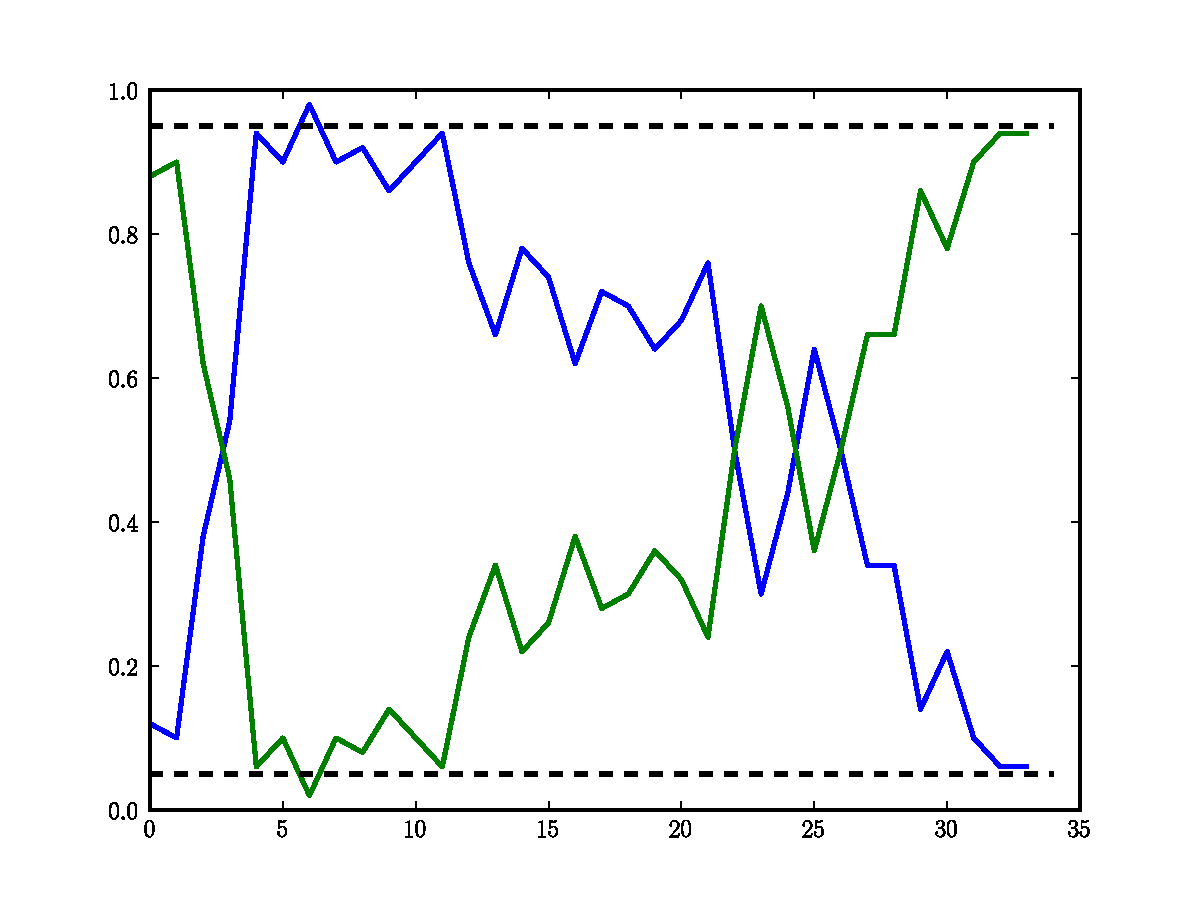
\includegraphics[width=\textwidth]{weights1.pdf}
\caption{Optimal arm probabilities for two arms.}
\label{fig:weights1}
\end{subfigure}
\begin{subfigure}[t]{.49\textwidth}
\centering
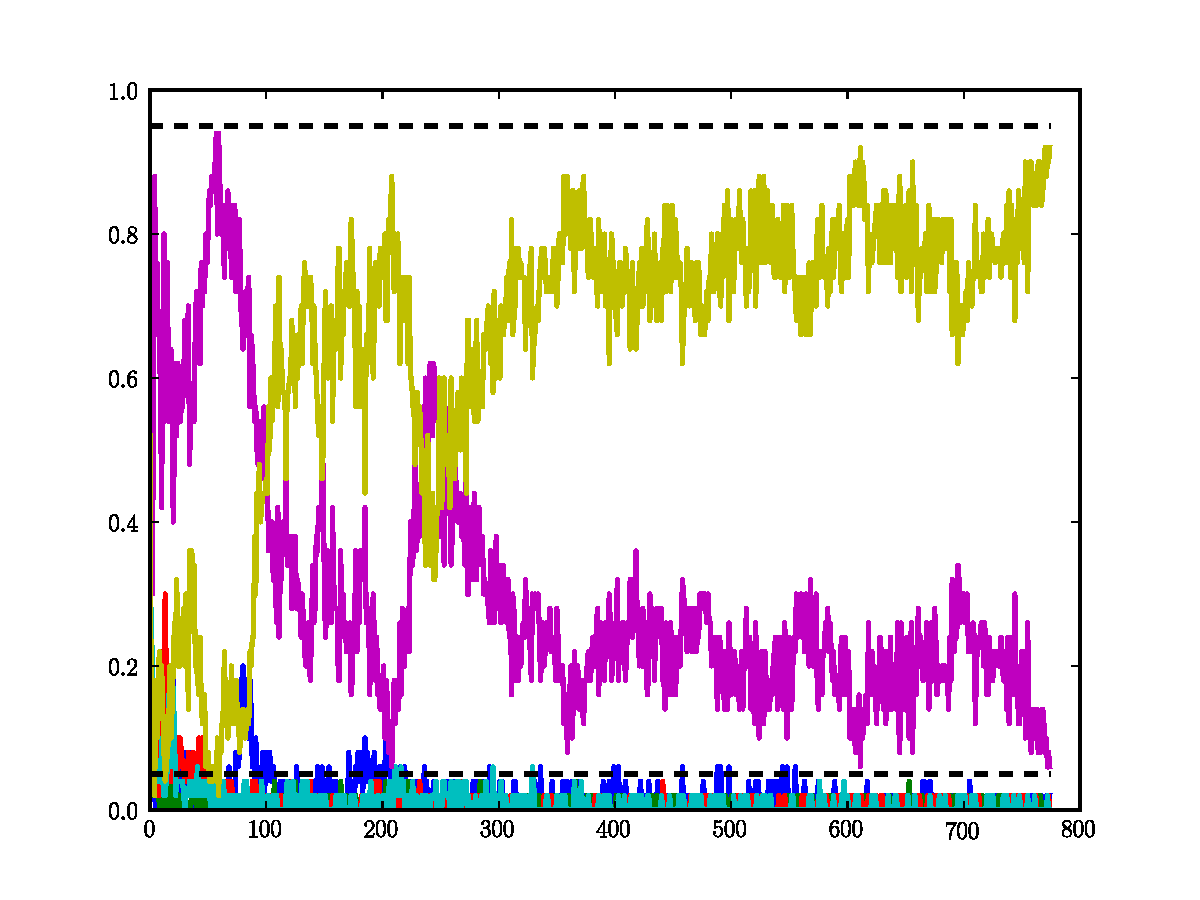
\includegraphics[width=\textwidth]{weights2.pdf}
\caption{Optimal arm probabilities for six arms.}
\label{fig:weights2}
\end{subfigure}
\end{figure}

% \begin{figure}[h]
% \centering
% 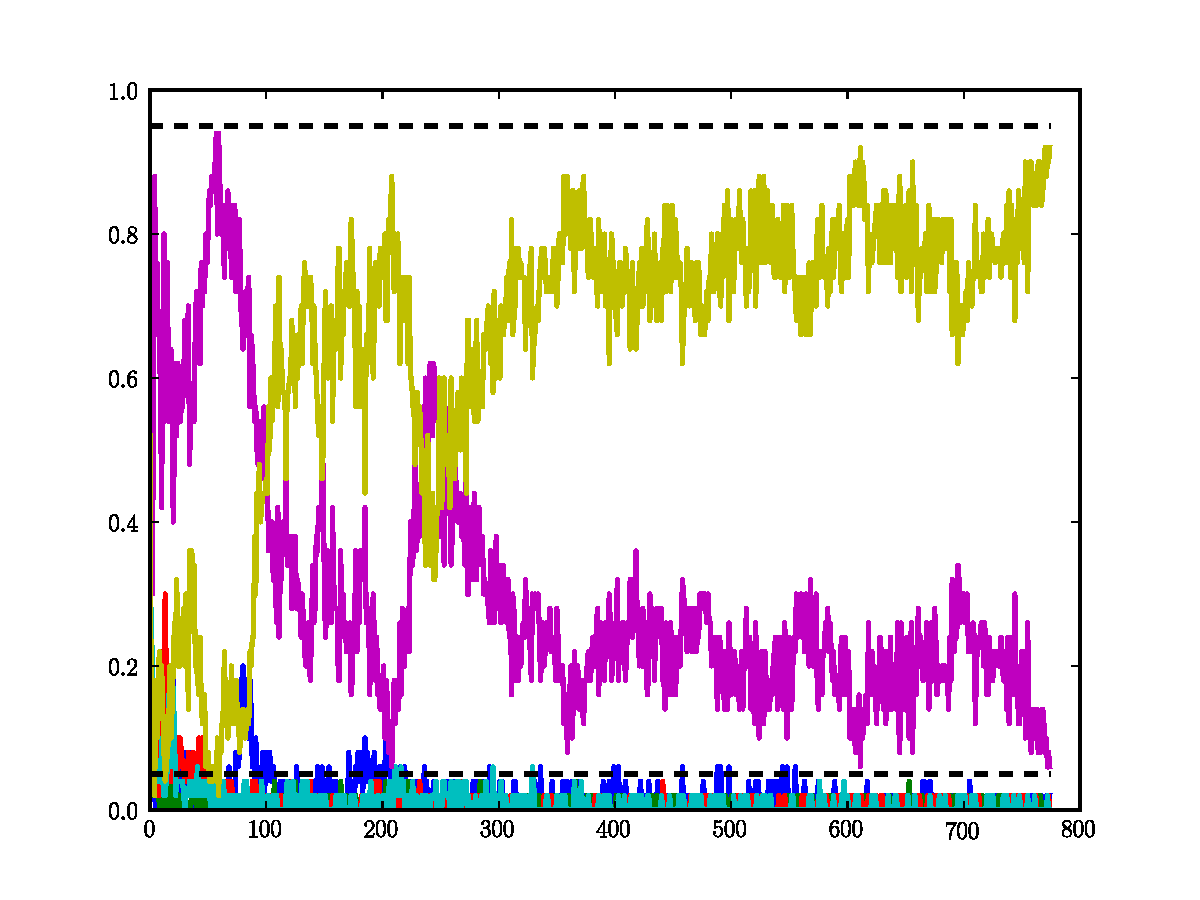
\includegraphics[width=\textwidth]{weights2.pdf}
% \caption{Optimal arm probabilities in the six arm case}
% \label{fig:weights2}
% \end{figure}


\section*{Comparison with Classical Tests}
A more classical approach to this problem would be to split traffic between each
variation for a predetermined amount of time, which should give enough data to
determine the best arm with some level of confidence.
Using the bandit approach described here has significant advantages over a classical test.
There are two main reasons why the bandit approach is more efficient.

The first reason is that the bandit method generally converges more quickly.
A standard test would require splitting the web page views between the different
variations over a long period of time.  According to Google's explanation in the
website mentioned at the beginning of this lab, the two arm case would take 223 days
and the 6 arm case would take 919 days.  The results from the simulations you performed
should show that on average the bandit method finishes much faster.
There are other ways we could choose our stopping criteria that may result in even shorter experiment times.
In general, we can always adjust the tolerance of our stopping criteria to shorten experiment time or increase accuracy.

The second reason the bandit approach is more efficient is that, as we gain more information,
we allocate more visits to the variation that we believe has a better CvR.
In the classical method we would split the visits evenly until the end of the experiment.
This way we gain many more conversions during testing than we would using classical tests.
